% \documentclass{article}[10pt]
% \usepackage[utf8]{inputenc}%characters and symbols from different languages
% \usepackage{graphicx} % Required for inserting images
% \usepackage[margin=1in]{geometry}
% \usepackage{amsfonts, amssymb, amsmath}
% \usepackage{tikz,pgfplots,hyperref}
% \usepackage{float}
% \usepackage{multirow}
% \usepackage{tabularx}
% \usepackage{hyperref}
% \usepackage{biblatex}% references package
% \usepackage{xcolor,colortbl}
% \title{Appendix}

% \begin{document}
% \maketitle
\chapter{Appendix}
%here we make tabkes from davids managment plan
\begin{table}[h!]
\begin{center}
    \begin{tabular}{ |c|c|c|c|c|c|c| }
    \hline
    &&\multicolumn{5}{c|}{Severity}\\
    \hline
    Probability of Occurence&&Negligible&Minor&Serious&Critical&Catastrophic\\
    \hline
    &Frequent&&&&&\\
    \hline
    &Probable&&&&&\\
    \hline
    &Occasional&&&&&\\
    \hline
    &Remote&&&&&\\
    \hline
    &Improbable&&&&&\\
    \hline
\end{tabular} 
\caption{Risk Assesibility}
\label{tab:Figure}

\end{center}
\end{table}
\begin{table}[h!]
    \begin{center}
        \begin{tabular}{ |c|c|c|c|c|c|c| }
        \hline
        &&\multicolumn{5}{c|}{Severity}\\
        \hline
        Probability of Occurence&&Negligible&Minor&Serious&Critical&Catastrophic\\
        \hline
        &Frequent&&&\cellcolor{gray}&\cellcolor{gray}&\cellcolor{gray}\\
        \hline
        &Probable&&&\cellcolor{gray}&\cellcolor{gray}&\cellcolor{gray}\\
        \hline
        &Occasional&&&&\cellcolor{gray}&\cellcolor{gray}\\
        \hline
        &Remote&&&&\cellcolor{gray}&\cellcolor{gray}\\
        \hline
        &Improbable&&&&\cellcolor{gray}&\cellcolor{gray}\\
        \hline
    \end{tabular} 
    \caption{Risk Assessment Criteria}
    \label{tab:Figure}
    
    \end{center}
    \end{table}
    The grey areas are areas where risks are not acceptable and will be eliminated or moved to 
    areas of less severity or occurrence probabilities. Since death and permanent impairments are not acceptable, 
    the two severity levels are not acceptable. Because the device should act in place of a lifeguard, it should not be 
    likely to cause further harm that require professional treatments, hence the partially unacceptable severity level “serious.” \\
    
\begin{table}[h!]
    \begin{center}
    \begin{tabular}{|c|c|}
        \hline
        Terms&Description\\
        \hline
        Negligible&Inconvenience or temporary discomfort\\
        \hline
        Minor  &Results in temporary impairment not requiring professional medical intervention\\
        \hline
        Serious&Results in temporary impairment requiring professional medical intervention\\
        \hline
        Critical&Results in permanent impairment or life-threatening injury\\
        \hline
        Catastrophic&Result in rescuer, rescuee, bystanders’ death\\
        \hline
    \end{tabular}
    \caption{Severity Levels Specifications}
    \label{tab:Figure}
\end{center}
\end{table}

\begin{table}[H]
    \begin{center}
    \begin{tabular}{|c|c|}
        \hline
        Terms&Description\\
        \hline
        Improbable&$<10^{-5}$\\
        \hline
        Remote&$<10^{-4}\; and \; \geq 10^{-5}$\\
        \hline
        Occasional&$<10^{-3} \;and \;\geq 10^{-4}$\\
        \hline
        Probable&$<10^{-2} \; and\; \geq 10^{-3}$\\
        \hline
        Frequent&$\geq 10^{-1}$\\
        \hline
    \end{tabular}
    \caption{Probability of Occurrence Specifications}
    \label{tab:Figure}
\end{center}
\end{table}   
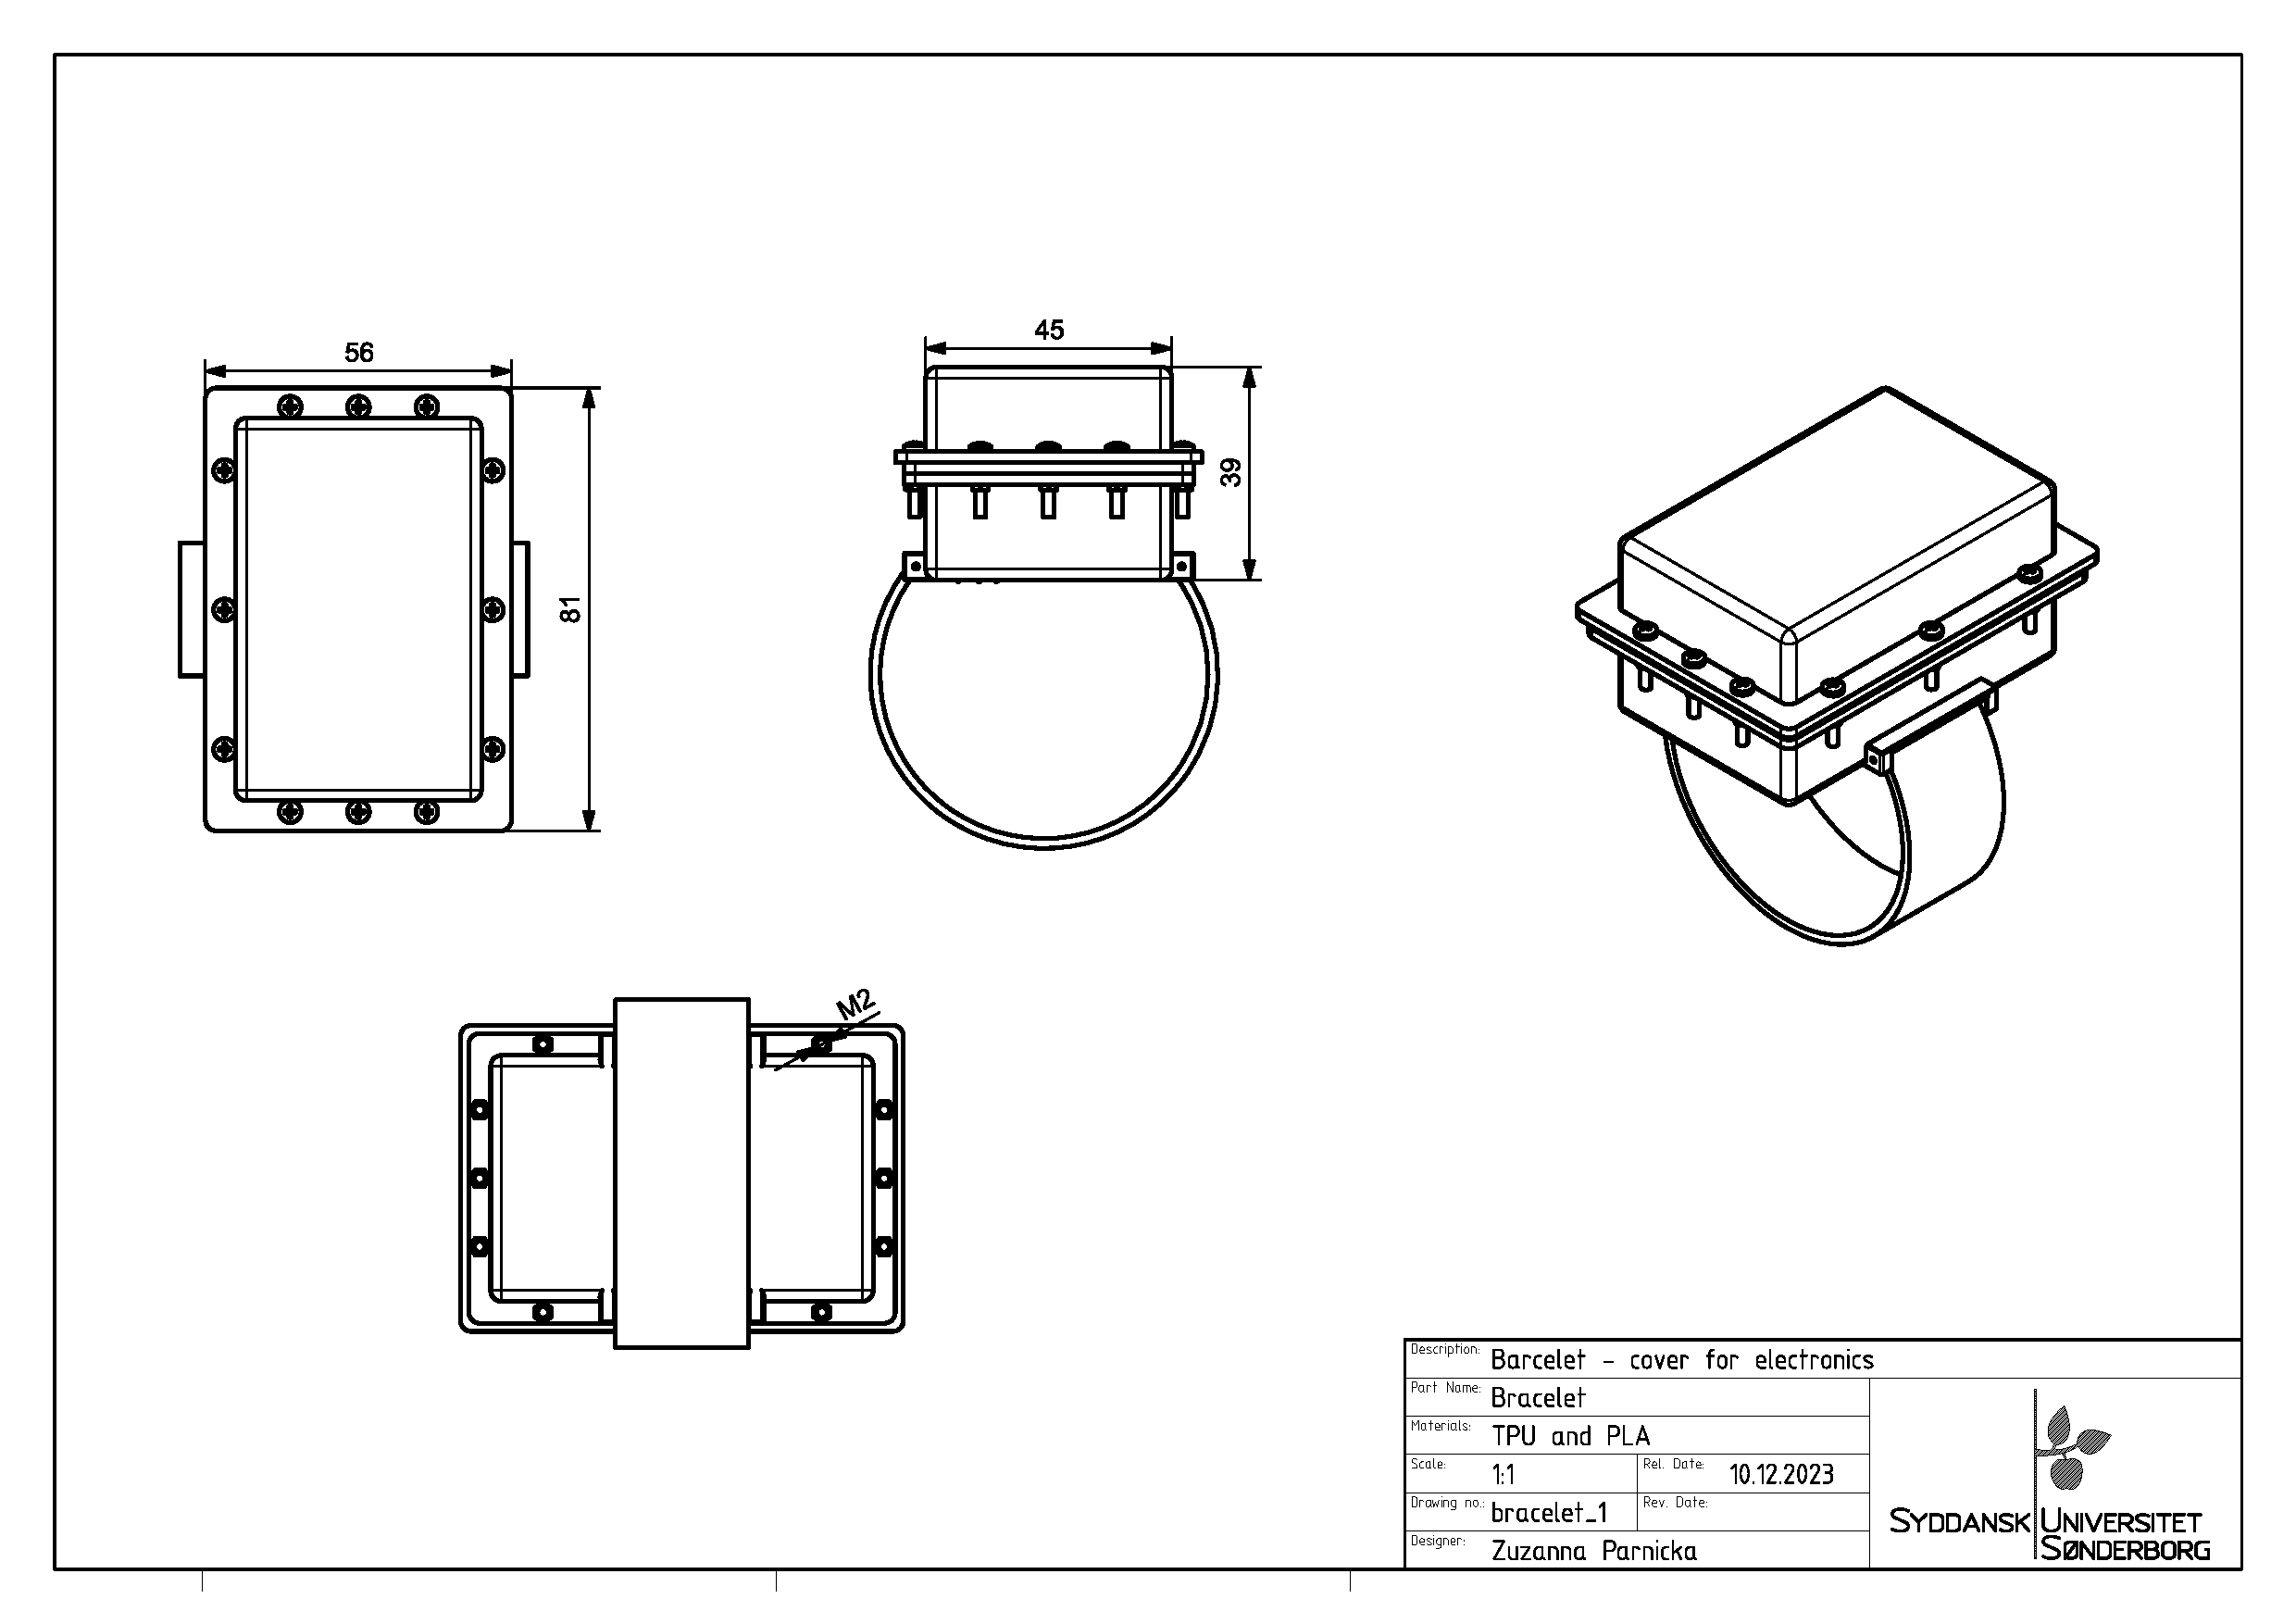
\includepdf[page=-]{bracelet_technical} 

% \end{document}